\section{Analisi Etnografica}
Un'applicazione può rivolgersi a diverse tipologie di utenti.
L'etereogenità di persone che al giorno d'oggi sono tecnologicamente in
grado di utilizzare smartphone e tablet è elevata, anche se va
considerato che esistono molteplici target d'utilizzo che si
differenziano per varie caratteristiche (e.g. fascie d'età, livello
d'istruzione, genere, stato civile, etc.).

Nello specifico, un'applicazione di cucina abbraccia sicuramente più di
una singola tipologia d'utente. 
Ad esempio ci si potrebbe aspettare un certo interesse verso tale applicazione
da utenti amanti della cucina con una predisposizione alla tecnologia, ma
anche da utenti poco informatizzati la cui gran passione per la cucina
li potrebbe portare a compiere lo sforzo di
apprendere il funzionamento di CookApp. \\

Identificare i diversi target d'utilizzo è fondamentale per comprendere
al meglio come strutturare un applicativo software, in quanto tipologie
di utenti divere si relazionano con esigenze diverse.

A tal proposito è stata condotta un'analisi etnografica che di seguito vedremo nel dettaglio. 

\subsection{Segmentazione del Target}
Al fine di individuare una categorizzazione di utenti in sottogruppi
omogenei per qualche caratteristica si fa fronte a due tipi di
segmentazione.

\subsubsection{Segmentazione Demografica}
Per comprendere meglio come segmentare l'utenza abbiamo considerato
attuali studi in letteratura che identificano caratteristiche
demografiche utili al nostro caso.
Nello specifico:
\begin{itemize}
\item Utilizzo demografico degli smartphone statutitesi nel 2014.
\begin{figure} [H]
	\centering
	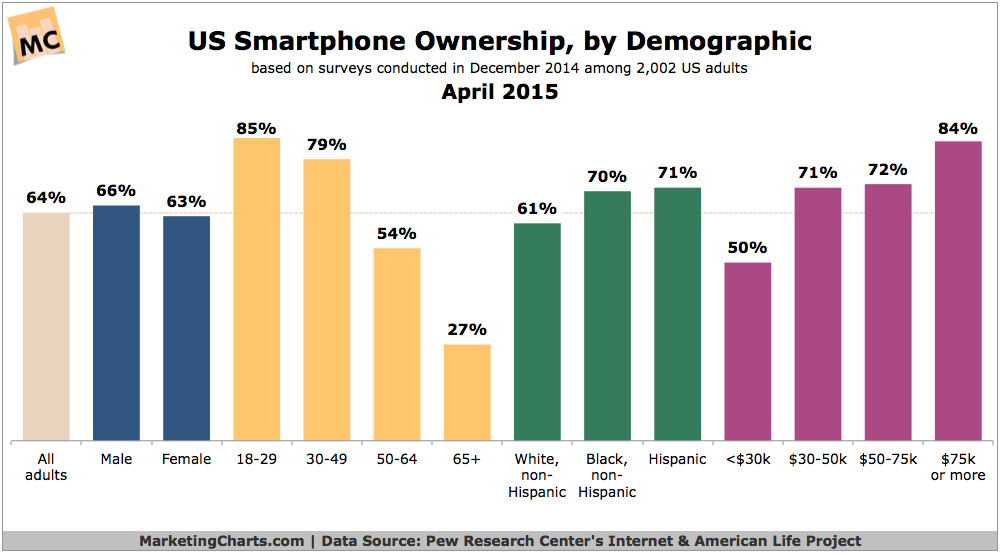
\includegraphics[scale=0.3]{img/demographic-smartphone.png}
\end{figure}
Dal grafico si envince che ormai l'utilizzo degli smartphone è
estremamente diffuso in quasi tutte le categorie demografiche.
I meno soggetti all'utilizzo di smartphone sono gli individui con un età
superiore ai 65 anni.

\begin{minipage}{0.45\textwidth}
\item
Crescita di interesse per la cucina.\\
Recenti articoli parlano di come
ci sia sempre più interesse verso l'arte culinaria. 
Si può riscontrare anche dal gran numero di programmi televisi in voga
negli anni. Inoltre si possono incontrare sempre più blog e canali
youtube nel web di appassionati di cucina che condividono le loro
ricette ed esperimenti.
La condivisione è una proprietà intrinseca della passione culinaria: le
nostre nonne hanno sempre conservato il libro delle ricette personali da
ampliare con le collezioni di ricette passate da amiche e parenti.
Indubbiamente questo fenomeno è esploso con il web e c'è sicuramente
spazio di mercato per applicazioni che permettono di coltivare la
passione culinaria.
\end{minipage}
\begin{minipage}{0.45\textwidth}
\begin{figure} [H]
	\centering
	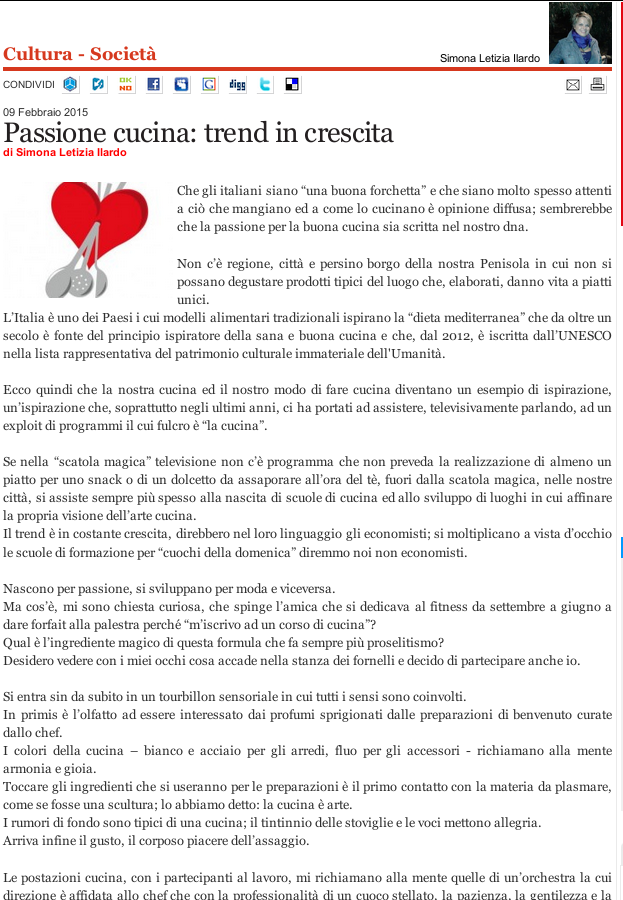
\includegraphics[scale=0.3]{img/articolo-cucina.png}
\end{figure}
\end{minipage}

La figura \ref{fig:demographic-cookapp} riassume uno studio statistico
condotto in Gran Bretagna nel 2013 che mostra la diffusione
dell'utilizzo di applicazioni per cucinare caratterizzata per età e
sesso. In particolare si può notare che c'è un maggiore utilizzo da
parte delle donne e da parte di persone sotto i 50 anni, anche se la
distribuzione è piuttosto omogenea.

\begin{figure}[H]
	\centering
	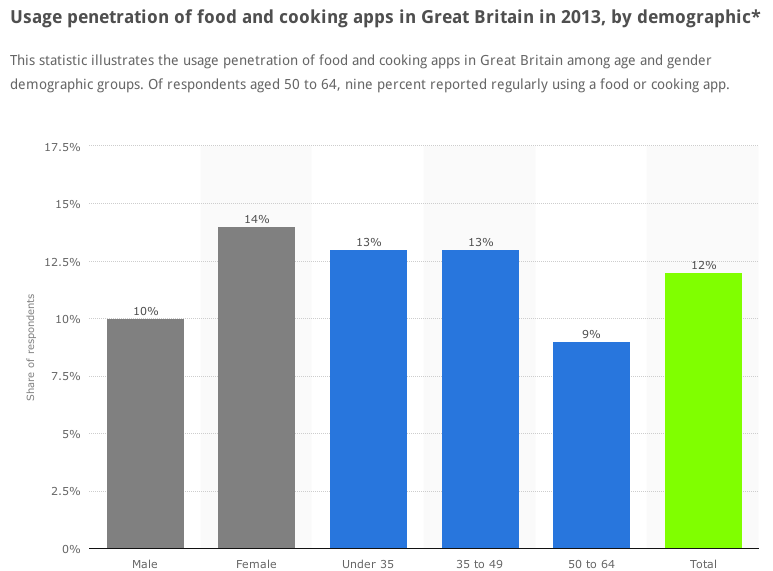
\includegraphics[scale=0.3]{img/demographic-cookapp.png}
	\caption{Diffusione demografica delle applicazioni culinarie in Gran Bretagna nel
2013}	
	\label{fig:demographic-cookapp}
\end{figure}

Inoltre come si evince dalla figura \ref{fig:cooking-country}, ci sono
nazioni in cui la passione per la cucina è molto importante a differenza di
altre. In particolare l'Italia risulta essere prima in classifica per
passione culinaria.
Questo suggerisce la possibilità di progettare un'applicazione culinaria
specifica per la cucina italiana, la quale da sé offre sicuramente un mercato
interessante, senza però escludere la possibilità di
coltivare la passione per la cucina internazionale. 
Un approccio meno specifico e più internazionale rischierebbe di
confondere l'utente medio italiano più legato ai ricettari classici
della cucina italiana. 

\begin{figure}[H]
	\centering
	
\includegraphics[scale=0.7]{img/cooking-country.jpg}
	\caption{Nazioni a confronto riguardo la passione culinaria}	
	\label{fig:cooking-country}
\end{figure}

\end{itemize}

Da quanto visto emerge un target ideale d'utilizzo che si differenzia per ogni
caratteristica demografica:
\begin{itemize}
\item \textbf{Età}. La fascia d'età di maggior interesse è dai 13-65
anni. Non esclude gli over 65 se con una particolare predisposizione
alla tecnologia.
\item \textbf{Sesso}. Qualsiasi: anche se le donne hanno mostrato avere più
interesse nella cucina rispetto agli uomini, il divario è minimo e rende
così l'applicazione indipendente dal sesso.
\item \textbf{Reddito}. Qualsiasi:
in genere le ricette presenti nelle applicazioni culinarie hanno diverse
fasce di prezzo rendendole di fatto indipendenti dal reddito dell'utente.
\item \textbf{Nazionalità}. Prevalentemente italiana. Non esclude gli
appassionati per la cucina italiana di diversa nazionalità.
\item \textbf{Istruzione}. È sufficiente possedere una cultura di base sulla terminologia
culinaria e sulla conoscenza delle materie prime più comuni. Si prevede
ovviamente che l'utente sia alfabetizzato e che comprenda le lingue
dell'applicazione. 

\end{itemize}

\subsubsection{Segmentazione Psicografica}
Al fine di identificare al meglio le tipologie di
utenti interessati all'applicazione proposta, abbiamo segmentato
ulteriormente l'utenza, in questo caso individuando le loro caratteristiche
psichiche.

\begin{itemize}
\item \textbf{Intraprendente}\\
L'applicazione potrebbe incuriosire quegli utenti che, nonostante il
basso livello di competenza tecnologica, non hanno paura di sperimentare
nuovi aspetti della vita quotidiana. In genere si parla degli
intraprendenti che, determinati ad ottenere una certa soluzione, non si
frenano davanti alle difficoltà.
\item \textbf{Insicuro}\\
Spesso si vedono amanti della cucina non molto abili dietro i fornelli,
a volte per lacune tecniche oppure perché mancano di sicurezza.
Quest'ultimi si riconoscono dalla minuziosità nel rispettare le dosi di
una ricetta e dalla paura di azzardare qualche punta di
personalizzazione.
Un'applicazione in grado di fornire delle ricette da cucina ad un alto
livello di dettaglio e suggerimenti su come poterle personalizzare,
sarebbe sicuramente attraente per gli utenti insicuri.
\item \textbf{Ansioso}\\
Solitamente le persone ansiose hanno difficoltà nell'organizzazione di
cene domestiche. Ad esempio può accadere che tali persone si portino troppo avanti
con le preparazioni per evitare di far attendere i loro ospiti, ma
potrebbero servire piatti freddi o eseguiti male se presi dal panico.
Un'applicazione che oltre a fornire delle ricette riesca anche a
pianificare dettagliatamente l'organizzazione di una cena potrebbe essere
interessante per gli utenti ansiosi.
\item \textbf{Curioso}\\
Spesso i buon gustai si chiedono come vengano preparati i loro piatti
preferiti. Questa è la categoria dei curiosi che potrebbero avvalersi di
un app da cucina per investigare sulle ricette che gli stuzzicano
l'interesse.
\item \textbf{Salutista}\\
Si vedono sempre più di frequente persone interessate a seguire un
alimentazione sana. In genere i salutisti sono coloro che fanno jogging
al parco, vanno in palestra tutti i giorni e stanno attenti alla linea.
La categoria però comprende anche coloro che, facendo poca attività
fisica, cercano di migliorare la loro qualità di vita con una dieta intenta 
a limitare la quantità di grassi assunti.
Per i salutisti un'applicazione che li guidi alla ricerca di ricette e
piatti compatibili con la loro alimentazione scelta potrebbe essere
molto interessante.

\end{itemize}


\subsection{User Research}
Con l'obiettivo di avere un'idea più chiara riguardo le caratteristiche
principali di usabilità dell'applicazione proposta, verrà analizzata di
seguito l'esito dell'attività di user research.

\subsubsection{Market Research}
Abbiamo preparato e pubblicato un sondaggio da far compilare ad un
insieme eterogeneo di persone. Abbiamo creato il questionario tramite
l'applicazione Google Form ed è stato compilato da 148
soggetti diversi.\\

Nello specifico riportiamo le domande e le relative risposte.
\begin{itemize}
	\item\textbf{Anagrafica}
		\begin{figure} [H]	
			\centering
			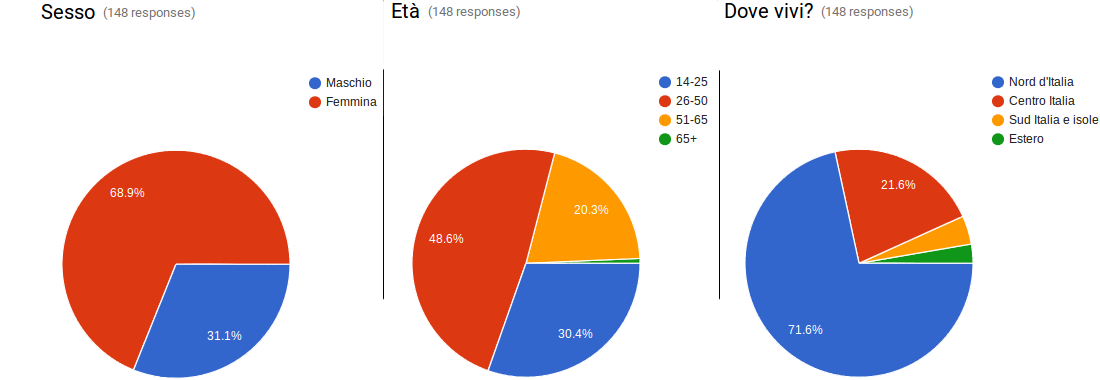
\includegraphics[width=\textwidth]{img/survey-123.png}
		\end{figure}
	\item\textbf{Competenze in Cucina}
		\begin{figure} [H]	
			\centering
			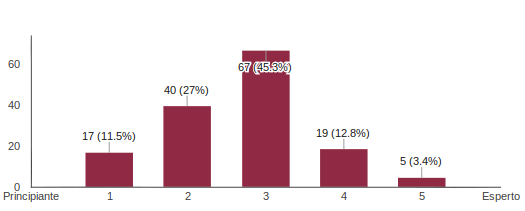
\includegraphics[scale=0.65]{img/survey-4.png}
		\end{figure}
	\item\textbf{Utilizzo Dispositivi in Generale}
		\begin{figure} [H]	
			\centering
			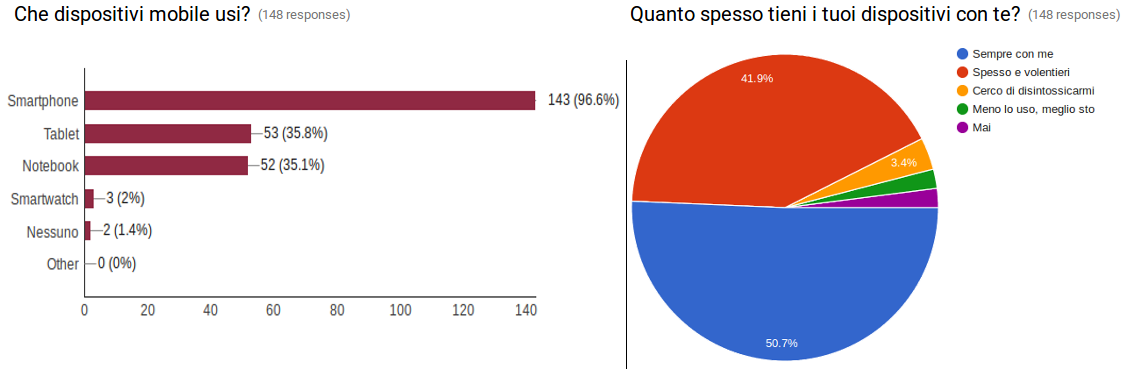
\includegraphics[scale=0.45]{img/survey-56.png}
		\end{figure}
	\item\textbf{Utilizzo Dispositivi in Cucina}
		\begin{figure} [H]
			\centering
			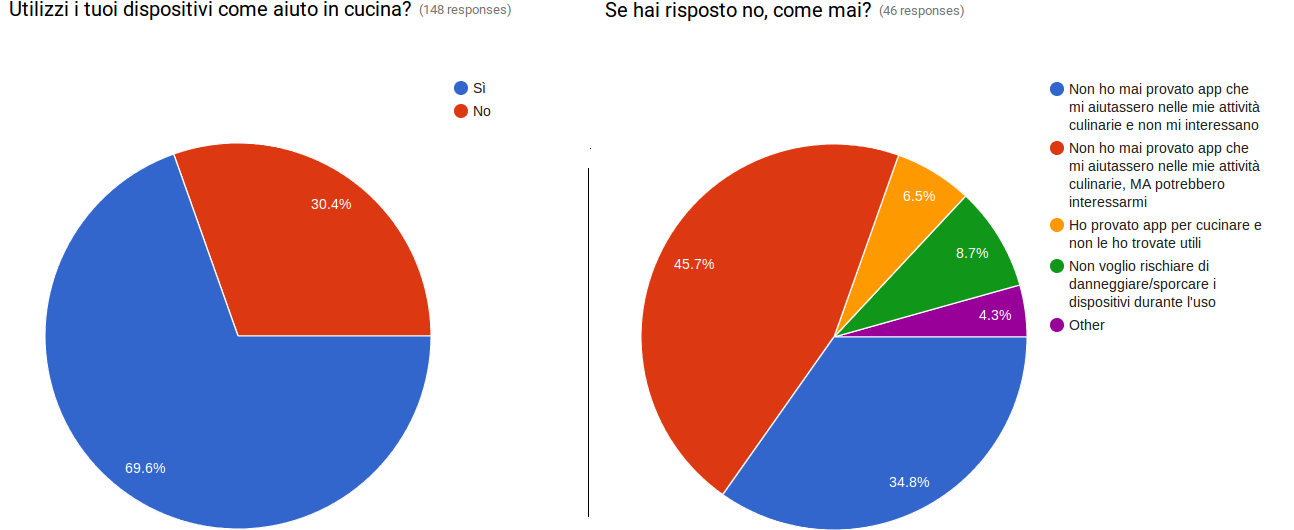
\includegraphics[scale=0.40]{img/survey-78.png}
		\end{figure}
		
		\begin{figure} [H]
			\centering
			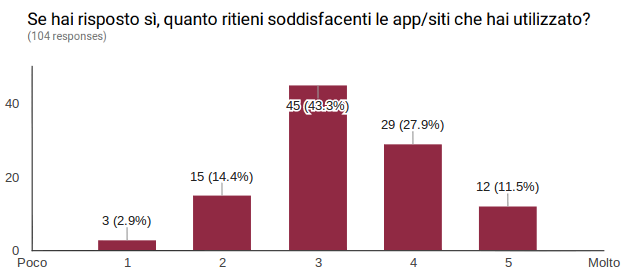
\includegraphics[scale=0.55]{img/survey-9.png}
		\end{figure}
	\item\textbf{Le funzioni che trovano o troverebbero più utili gli
utenti in un app per cucinare}\\
		Le risposte possibili erano le seguenti:
		\begin{enumerate}
			\item Un buon catalogo di ricette
			\item Le video ricette
			\item I consigli della community
			\item La possibilità di creare liste della spesa di ricette
			\item La possibilità di organizzare un pasto completo
tramite l'abbinamento di ricette
			\item La possibilità di controllare i procedimenti tramite
comandi vocali
			\item Altro (risposta libera)
		\end{enumerate}
		\begin{figure} [H]
			\centering
			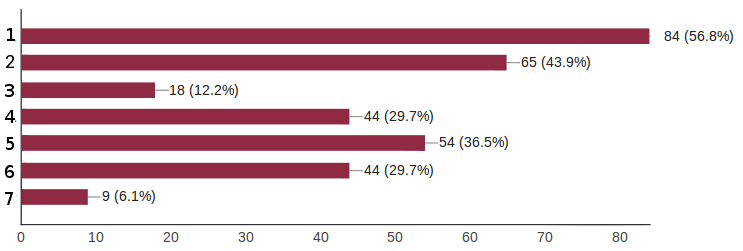
\includegraphics[scale=0.55]{img/survey-10.png}
		\end{figure}
	Le proposte più interessanti tra quelle a risposta libera sono
state: ``La possibilità di ricavare ricette dagli ingredienti
disponibili'' e ``La possibilità di scegliere le ricette in base a
intolleranze'' la quale è stata proposta da più utenti anche se in forme
leggermente diverse.
	\item \textbf{Lista della spesa}
		\begin{figure} [H]
			\centering
			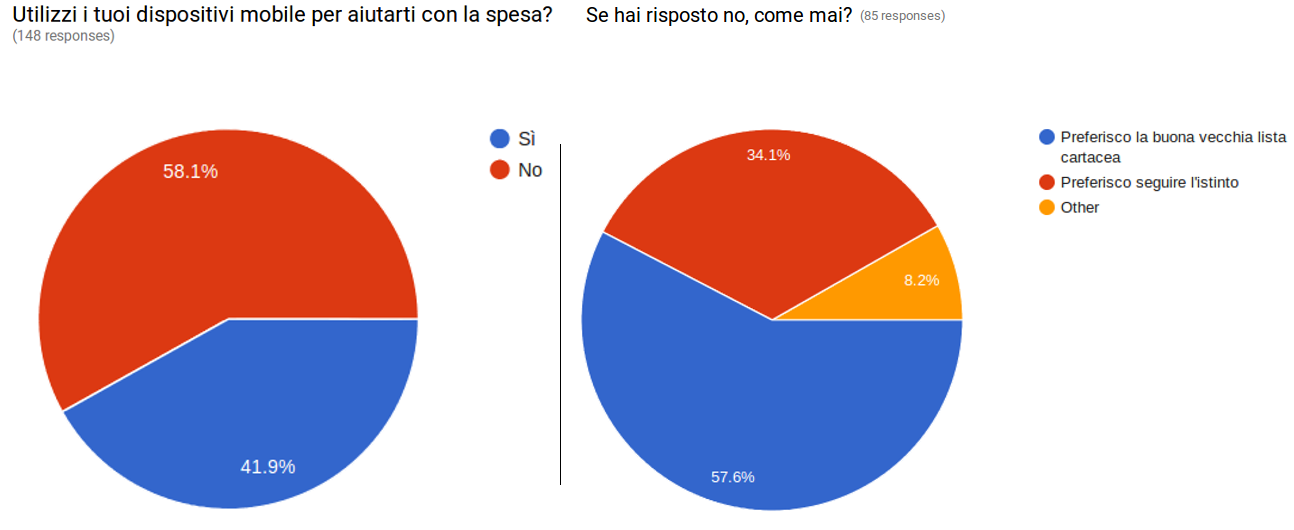
\includegraphics[scale=0.40]{img/survey-1112.png}
		\end{figure}
	Nelle spiegazioni alle risposte negative, la maggior parte delle
persone che ha risposto "Altro" ha indicato che in genere non
utilizza affatto liste delle spesa.
\end{itemize}

Sommariamente il sondaggio ha coinvolto un gruppo di persone di sesso
prevalentemente
femminile, età principalmente dai 14-50 anni e concentrati
nel nord e centro Italia.\\
Il pool di esaminati ha definito mediamente di avere competenze culinarie
medio-basse e come aspettato di essere molto dipendete dai dispositivi
mobili più comuni in commercio. \\

Inoltre, circa il 70\% di loro ha dichiarato di
utilizzare tali dispositivi come aiuto in cucina trovandole mediamente
soddisfacenti. Il restante
30\% invece non utilizza dispositivi mobili in cucina, ma 
quasi la metà di loro sarebbe interessata ad utilizzarli non avendo però
mai provato applicazioni per cucinare.
In aggiunta, gli esaminati trovano estremamente interessante
applicazioni che offrono un buon catalogo di ricette e video ricette.
Scaturiscono anche discreto interesse funzionalità per creare liste
della spesa, organizzare menù completi abbinando più ricette e il
controllo dell'applicazione tramite comandi vocali. Invece viene presa
poco in considerazione il supporto da parte della community.
Infine i soggetti esaminati si dividono quasi per le metà tra chi
utilizza dispositivi mobili per fare la spesa e chi invece no, con una
piccola prevalenza per questi ultimi.\\

Da questa ricerca di mercato si evince che c'è sicuramente domanda per
questo tipo di applicazioni e margine di miglioramento rispetto ai prodotti
già esistenti considerando i livelli di soddisfazione delle persone
esaminate.
\subsubsection{Contextual Inquiry}
Vedremo qui di seguito due osservazioni effettuate sul campo d'azione
di alcuni potenziali utenti, al fine di individuare dettagli importanti
dipendenti dal contesto d'utilizzo dell'applicazione.

\begin{enumerate}
\item Dario, Paolo e Giacomo sono tre coinquilini universitari, svegli ma non molto
abili in cucina. Nonostante la loro poca esperienza, occasionalmente
decidono di cimentarsi nella preparazione di qualche ricetta trovata
online, sia per rompere la monotonia della classica pasta con il tonno,
sia per avere una valida distrazione dallo studio.
Sono stati osservati nel tentativo di preparazione di un dolce.
Inizialmente i tre hanno deciso di far pranzo con delle
tagliatelle all'arancia, una delle prime ricette trovate online che ha risvegliato il
loro appetito. Seguendo nel dettaglio la ricetta hanno portato a termine
con successo la preparazione delle tagliatelle gustandosi un buon
pranzo insolito. 
Quella mattina però al supermercato non vendevano
arance sfuse e hanno dovuto per forza acquistare la confezione grande.
Inoltre la ricetta delle tagliatelle prevedeva l'utilizzo di soltanto i
tuorli delle uova così che i tre studenti si sono ritrovati con un
eccesso di arance e albumi dopo il pranzo.

Mossi dalla loro grande voracità e dall'alternativa di un triste pomeriggio sui libroni di
matematica hanno deciso di cercare online un dolce all'arancia.
Hanno deciso quindi di tentare la preparazione di una mousse
all'arancia. La ricetta richiedeva però la colla di pesce, ingredienti non di uso
quotidiano per tre studenti universitari abituati ad ordinare persino il
dolce a domicilio. Troppo sicuri delle loro intuizioni hanno però
provato lo stesso a preparare la mousse utilizzando gli albumi montati a
neve in sostituzione alla colla di pesce. 

Al termine della preparazione hanno preso atto che la consistenza non era adatta ad una mousse. 
Hanno deciso quindi di aggiungere del cacao amaro in
polvere al composto senza alcuna ragione reale ma spinti piuttosto dalla curiosità e divertiti
dall'improvvisazione. Mescolando però ulteriormente l'impasto hanno smontato
gli albumi. A quel punto affranti dall'eventualità di non poter gustare
alcun dolce hanno deciso di ripiegare disperati su una torta
``facciopresto'' consigliata telefonicamente da una loro amica. Hanno
quindi infine aggiunto farina e burro all'impasto e infornato il tutto
ottenendo in ultimo un risultato qualitativamente molto scarso.
Ovviamente Dario, Paolo e Giacomo, ormai stanchi e affamati, hanno comunque consumato interamente la
torta non desiderata, sognando ad ogni morso una deliziosa mousse all'arancia.

\item Antonietta è un'impiegata di 48 anni del sud Italia. È una signora che
nella sua vita ha viaggiato poco ed è molto legata alle tradizioni della
sua terra d'origine. Da quando i suoi figli hanno lasciato casa per
studio e lavoro, Antonietta ha iniziato ad interessarsi di più alla
ricerca culinaria e alla sperimentazione di piatti che si distaccassero
dalle sue tradizioni.\\

La signora Antonietta è stata osservata durante la preparazione della polenta taragna, un
piatto tipico valtellinese la cui ricetta è stata da lei trascritta dopo
averne visto la preparazione in un programma culinario televisivo.

Antonietta inizia la preparazione del piatto seguendo minuziosamente le
dosi della ricetta e pesando nel dettaglio ogni ingrediente. Casualmente
quel giorno era in casa anche sua sorella Roberta che ha un amica,
Elisa, originaria del nord Italia trasferitasi in Puglia dopo il matrimonio.
Roberta ha visto una volta preparare la polenta taragna da Elisa e
ricorda che per la preparazione della polenta taragna occorrono circa 5
bicchieri di farina per una forma piccola di formaggio. La signora
Antonietta non si fida molto della memoria e della sicurezza di sua sorella
e vuole procedere per la strada della ricetta. Le due discutono per
diverso tempo sul corrispettivo in grammi di 5 bicchieri di farina e su
sul tipo di bicchieri da prendere in considerazione per tale
conversione. Fanno anche diverse prove con vari bicchieri in quanto la
signora Antonietta non aveva lo stesso identico modello di bicchieri della
signora Elisa. Infine Antonietta perde la pazienza e continua per la sua
strada utilizzando il dosaggio in grammi indicato nella ricetta. La
preparazione del piatto viene terminata con successo e con un'ottima
polenta taragna, anche se le due sorelle non la gustano al meglio avendo
gli animi ancora alterati dalla precedente discussione.
\end{enumerate}

Analizzando le due osservazioni emergono dei dettagli di usabilità da
tenere in considerazione.

Nel caso dei tre studenti una buona
applicazione avrebbe potuto suggerire un ingrediente opportuno in
sostituzione alla colla di pesce. Inoltre con la possibilità di chiedere
aiuto alla community, l'app avrebbe dato la possibilità ai tre ragazzi di capire in
anticipo che gli albumi delle uova montati a neve non sono opportuni per
una mousse sotto suggerimento di qualche altro utente.

Per quanto riguarda la signora Antonietta, se avesse usato un'applicazione 
da cucina con una funzionalità di conversione da grammi a
bicchieri, avrebbe evitato di discutere con la sorella. In
alternativa avrebbe anche potuto chiedere conferma agli
utenti valtellinesi della community della correttezza delle dosi scritte
nella ricetta.

\subsubsection{Task Analisys}
Dalla ricerca di mercato e dall'analisi del contesto si sono individuate
le attività che vengono e che potrebbero venir svolte durante l'utilizzo
di un applicazione da cucina. È stata rivolta particolare attenzione
alle risposte del survey, che già in parte indirizzano verso le
funzionalità richieste dall'utente, e alle osservazioni del contextual
inquiry che indicano già una possibile sequenza di passi che gli utenti
compiono durante la preparazione di una ricetta.
È stata quindi definita la seguente lista di task:
\begin{enumerate}
\label{tasks}
\item Con l'intento di preparare un pasto completo per più persone,
l'utente dell'applicazione deve individuare tutte le ricette d'interesse
facendo particolarmente attenzione ai tempi di cottura, le difficoltà di
preparazione e la lista di ingredienti necessari.
\item Durante il periodo natalizio l'utente vuole preparare un dessert a tema
e condividere una recensione finale con foto sui social network.
\item L'utente ha ideato una rivisitazione di un piatto del suo chef
preferito e vuole inserirne la ricetta nel catalogo dell'applicazione.
Infine decide inserire la ricetta nei propri preferiti al fine di non
dimenticarla più.
\item L'utente durante la stesura della pasta fresca non vuole
interagire fisicamente con il suo nuovissimo dispositivo, dati i
sacrifici economici richiesti per l'acquisto. Quindi vuole utilizzare
comandi vocali e guida vocale  per portare a termine la preparazione del
piatto.
\item Dopo aver individuato una ricetta d'interesse, l'utente vuole
inserire nella lista della spesa digitale gli ingredienti necessari.
\end{enumerate}

Vedremo in seguito gli approcci delle applicazioni già esistenti verso
questi task e le funzionalità da progettare nella nostra applicazione
affinché tali task possano essere eseguiti al meglio.
